\documentclass[11pt]{article}
\usepackage[T1]{fontenc}
\usepackage[utf8]{inputenc}
\usepackage[a4paper,margin=1in]{geometry}
\usepackage{lmodern}
\usepackage{amsmath,amssymb,mathtools}
\usepackage{booktabs,longtable,array}
\usepackage{enumitem}
\usepackage{graphicx}
\usepackage{xcolor}
\usepackage{float}
\usepackage{hyperref}
\usepackage{tikz}
\usetikzlibrary{arrows.meta,positioning,shapes.geometric,calc,fit}
\hypersetup{colorlinks=true,linkcolor=blue!50!black,urlcolor=blue!50!black}

\title{Forecasting Future Fluorescence Expression\\from Early Brightfield Organoid Imaging}
\author{OrganoidAgent Yichao Forecasting Design}
\date{2026-05-10}

\newcommand{\R}{\mathbb{R}}
\newcommand{\1}{\mathbf{1}}
\newcommand{\E}{\mathbb{E}}
\newcommand{\argmin}{\operatorname*{arg\,min}}
\newcommand{\argmax}{\operatorname*{arg\,max}}
\newcommand{\median}{\operatorname{median}}
\newcommand{\MAD}{\operatorname{MAD}}
\newcommand{\IoU}{\operatorname{IoU}}
\newcommand{\AUROC}{\operatorname{AUROC}}
\newcommand{\AUPRC}{\operatorname{AUPRC}}
\newcommand{\SmoothLone}{\operatorname{SmoothL1}}

\begin{document}
\maketitle
\tableofcontents

\section{Goal}
The practical goal is not only to translate a same-time brightfield image into a same-time fluorescence image. The real biological goal is to predict later fluorescence expression before the organoid visibly expresses fluorescence.

There are therefore two related tasks:
\begin{enumerate}[leftmargin=1.5em]
  \item \textbf{Same-time translation:} learn \(B_t \mapsto F_t\), where \(B_t\) is brightfield and \(F_t\) is fluorescence at the same time and depth.
  \item \textbf{Future forecasting:} learn \(B_{1:k} \mapsto Y_{>k}\), where \(B_{1:k}\) is an early brightfield history before detectable expression and \(Y_{>k}\) summarizes future fluorescence expression.
\end{enumerate}

The second task is the target method. Same-time pix2pix remains useful because it validates image registration, channel pairing, segmentation quality, and whether morphology contains immediate fluorescence-related information. It does not by itself solve future prediction.

\section{Channel Convention}
The current instance-pair segmentation/database pipeline uses:
\begin{itemize}[leftmargin=1.5em]
  \item \(c1\): brightfield input,
  \item \(c0\): fluorescence target.
\end{itemize}

Some older notes used the opposite wording. Before training any model, verify the channel by opening paired files such as:
\begin{verbatim}
*_t000_z000_c1.jpg  brightfield
*_t000_z000_c0.jpg  fluorescence
\end{verbatim}

\section{Which Data Can Be Used}
\subsection{Find datasets with time information first}
Future forecasting requires time-indexed data. A static one-frame image can train same-time translation, but it cannot answer whether early morphology predicts later expression.

The exported Yichao filenames have this form:
\begin{verbatim}
<series>_<object_name>_tTTT_zZZZ_cC.jpg
\end{verbatim}

A folder has time information if at least one object has more than one unique \(t\)-index:
\begin{equation}
T_{\mathrm{object}} =
\left|\left\{t : \exists z,c \;\mathrm{file}(object,t,z,c)\right\}\right| > 1 .
\end{equation}

For paired supervised data, the brightfield and fluorescence files must share the same object, time, and depth:
\begin{equation}
(B_{p,t,z},F_{p,t,z}) =
\left(I_{p,t,z,c=1}, I_{p,t,z,c=0}\right),
\end{equation}
where \(p\) denotes the position or object folder.

\subsection{Real Yichao time-aware inventory}
Table~\ref{tab:data-inventory} summarizes the current usable Yichao folder structure discovered from the grouped JPEG roots. Pair counts are 2D paired planes, not organoid-instance counts.

\begin{longtable}{@{}llrrrrl@{}}
\caption{Yichao paired-frame inventory. \(T_{\max}\) and \(Z_{\max}\) are the maximum number of timepoints and z-planes observed in a position.}\label{tab:data-inventory}\\
\toprule
Dataset & Main role & Pairs & Positions & \(T_{\max}\) & \(Z_{\max}\) & Day tags\\
\midrule
\endfirsthead
\toprule
Dataset & Main role & Pairs & Positions & \(T_{\max}\) & \(Z_{\max}\) & Day tags\\
\midrule
\endhead
Data-Yichao-1 & static check only & 5 & 5 & 1 & 1 & none\\
Data-Yichao-2 & dynamic D2 plus duplicated static images & 965 & 11 & 16 & 11 & D2\\
Data-Yichao-3 & dynamic monitoring & 10019 & 13 & 49 & 32 & Day 2--4\\
Data-Yichao-4 & dynamic monitoring & 7940 & 9 & 49 & 38 & Day 2--3\\
Data-Yichao-5 & dynamic monitoring & 10143 & 12 & 45 & 34 & D1--D3\\
Data-Yichao-6 & dynamic D4 monitoring & 4410 & 3 & 45 & 40 & D4\\
Data-Yichao-7 & dynamic D1--D3 monitoring & 7706 & 8 & 38 & 39 & D1--D3\\
Data-Yichao-8 & dynamic D2--D3 monitoring & 12536 & 18 & 45 & 36 & D2--D3\\
Data-Yichao-9 & PDO28/Jurkat live imaging & 4756 & 3 & 116 & 15 & D2--D3\\
Data-Yichao-10 & dynamic monitoring & 16605 & 13 & 41 & 46 & DF\\
\bottomrule
\end{longtable}

For the forecasting task, prioritize datasets with clear time courses and repeated positions:
\begin{itemize}[leftmargin=1.5em]
  \item first: Data-Yichao-3, 4, 5, 7, 8, 10;
  \item optional after inspection: Data-Yichao-2 dynamic D2 positions and Data-Yichao-6 D4 positions;
  \item separate biological task: Data-Yichao-9 because it contains PDO28/Jurkat live imaging and T-cell fluorescence.
\end{itemize}

\subsection{Concrete examples for datasets 6--8}
The currently processed set \(6,7,8\) contains exactly the kind of time/depth structure needed for a future model:
\begin{itemize}[leftmargin=1.5em]
  \item Data-Yichao-6: 3 D4 positions, 45 timepoints, 25--40 z-planes.
  \item Data-Yichao-7: 8 positions across D1, D2, D3, 31--38 timepoints, 17--39 z-planes.
  \item Data-Yichao-8: 18 positions across D2 and D3, 32--45 timepoints, 9--36 z-planes.
\end{itemize}

The most useful forecasting subset is any same-position or same-condition sequence where early frames precede fluorescence onset and later frames contain expression.

\section{Recommended Data Representation}
\subsection{Frame-level pair}
The lowest-level pair is:
\begin{equation}
\mathcal{P}_{p,t,z} = (B_{p,t,z},F_{p,t,z}).
\end{equation}
This pair is enough for same-time pix2pix, but it is not enough for forecasting.

\subsection{Instance-level pair}
After segmentation, every organoid instance \(i\) has:
\begin{equation}
\mathcal{I}_{i,p,t,z} =
\left(B_{i,p,t,z}^{\mathrm{crop}},
F_{i,p,t,z}^{\mathrm{crop}},
M_{i,p,t,z},
m_{i,p,t,z}\right),
\end{equation}
where \(M\) is the mask and \(m\) is a vector of morphology features.

For the first forecasting model, keep only complete instances:
\begin{equation}
\mathrm{complete}(i,p,t,z) = \1[\mathrm{is\_edge\_padded}=0].
\end{equation}

\subsection{Track-level sample}
The correct forecasting unit is an organoid track:
\begin{equation}
\mathcal{T}_j =
\left\{
\left(B_{j,t}^{\mathrm{crop}},F_{j,t}^{\mathrm{crop}},M_{j,t},m_{j,t}\right)
\right\}_{t=1}^{T_j}.
\end{equation}

Here \(j\) indexes a physical organoid tracked through time. In practice, \(B_{j,t}\) should be a 2D representation per timepoint, not a full z-stack at first. Good first choices are:
\begin{itemize}[leftmargin=1.5em]
  \item central z-plane,
  \item best-focus z-plane,
  \item max or mean projection,
  \item one stable z-plane if the z-index is biologically meaningful.
\end{itemize}

\section{Pipeline Flow}
\begin{figure}[H]
\centering
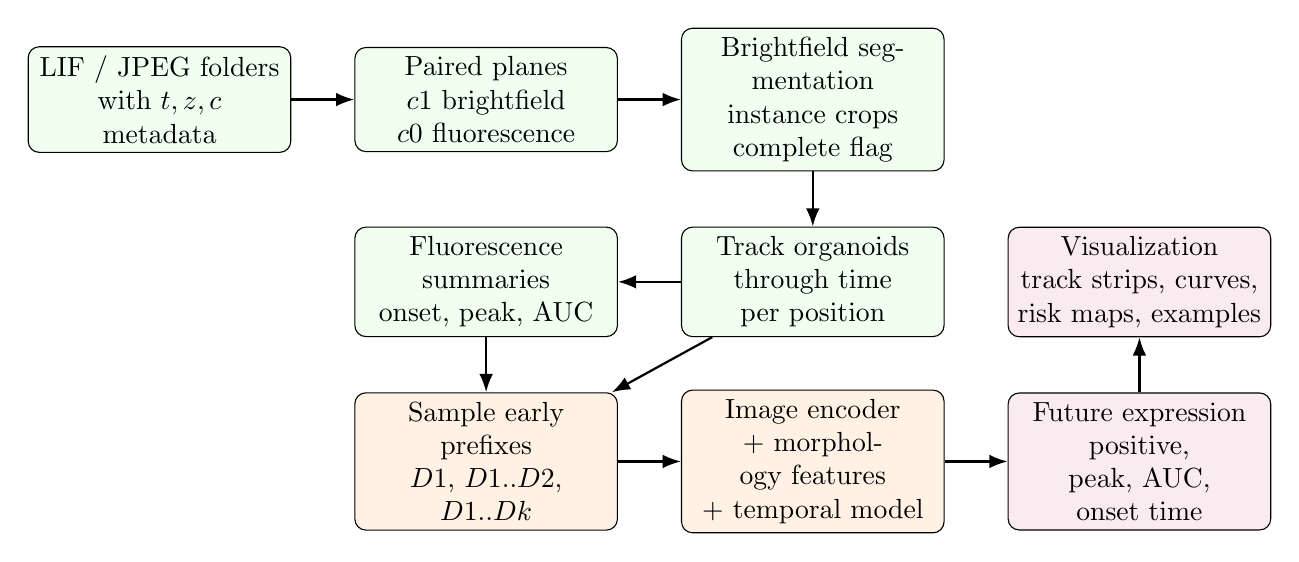
\begin{tikzpicture}[
  node distance=7mm and 8mm,
  box/.style={draw, rounded corners, align=center, minimum height=8mm, text width=31mm, fill=blue!5},
  data/.style={draw, rounded corners, align=center, minimum height=8mm, text width=31mm, fill=green!6},
  model/.style={draw, rounded corners, align=center, minimum height=8mm, text width=31mm, fill=orange!10},
  resultbox/.style={draw, rounded corners, align=center, minimum height=8mm, text width=31mm, fill=purple!8},
  arrow/.style={-Latex, thick}
]
\node[data] (lif) {LIF / JPEG folders\\with \(t,z,c\) metadata};
\node[data, right=of lif] (pairs) {Paired planes\\\(c1\) brightfield\\\(c0\) fluorescence};
\node[data, right=of pairs] (seg) {Brightfield segmentation\\instance crops\\complete flag};
\node[data, below=of seg] (track) {Track organoids\\through time\\per position};
\node[data, left=of track] (onset) {Fluorescence summaries\\onset, peak, AUC};
\node[model, below=of onset] (prefix) {Sample early prefixes\\\(D1\), \(D1..D2\),\\\(D1..Dk\)};
\node[model, right=of prefix] (encoder) {Image encoder\\+ morphology features\\+ temporal model};
\node[resultbox, right=of encoder] (pred) {Future expression\\positive, peak, AUC,\\onset time};
\node[resultbox, above=of pred] (viz) {Visualization\\track strips, curves,\\risk maps, examples};

\draw[arrow] (lif) -- (pairs);
\draw[arrow] (pairs) -- (seg);
\draw[arrow] (seg) -- (track);
\draw[arrow] (track) -- (onset);
\draw[arrow] (onset) -- (prefix);
\draw[arrow] (prefix) -- (encoder);
\draw[arrow] (encoder) -- (pred);
\draw[arrow] (pred) -- (viz);
\draw[arrow] (track) -- (prefix);
\end{tikzpicture}
\caption{Forecasting pipeline from real Yichao time-indexed image folders to future expression predictions.}
\label{fig:pipeline}
\end{figure}

\section{Tracking}
\subsection{Simple first tracker}
For every position \(p\), timepoint \(t\), and chosen z representation, the segmentation pipeline produces instances \(a\in A_t\) and \(b\in A_{t+1}\). Link them by minimizing a cost:
\begin{equation}
C(a,b) =
\lambda_d \frac{\lVert c_a-c_b\rVert_2}{r_a+r_b+\epsilon}
\lambda_o \left(1-\IoU(M_a,M_b)\right)
\lambda_s \left|\log\frac{A_a+\epsilon}{A_b+\epsilon}\right|,
\end{equation}
where \(c\) is centroid, \(r\) is equivalent radius, \(M\) is mask, and \(A\) is mask area.

Use Hungarian matching or greedy nearest-neighbor matching under a maximum cost threshold:
\begin{equation}
(a,b)\;\mathrm{is\;linked}\quad\Longleftrightarrow\quad
b=\argmin_{b'\in A_{t+1}} C(a,b') \;\;\mathrm{and}\;\; C(a,b)<\tau_{\mathrm{track}}.
\end{equation}

Break a track if no confident match exists. Keep tracks satisfying:
\begin{equation}
T_j^{\mathrm{early}}\ge T_{\min}^{\mathrm{early}},
\qquad
T_j^{\mathrm{future}}\ge T_{\min}^{\mathrm{future}},
\qquad
\mathrm{complete}(j,t)=1 \;\mathrm{for\ most\ frames}.
\end{equation}

\subsection{Why not full 3D tracking first}
Full 3D tracking is possible but not the best first implementation. The early goal is to learn whether brightfield morphology predicts later expression. A stable 2D projection or best-focus plane is easier to validate and less sensitive to z-plane noise.

\section{Fluorescence Signal and Onset}
\subsection{Background-corrected fluorescence}
For each track \(j\) and time \(t\), define the organoid mask \(M_{j,t}\) and a local background ring \(R_{j,t}\) around the organoid. A robust fluorescence score is:
\begin{equation}
S_{j,t} =
\operatorname{quantile}_{0.90}\left(F_t(x):x\in M_{j,t}\right)
-
\median\left(F_t(x):x\in R_{j,t}\right).
\end{equation}

Also compute:
\begin{align}
\bar{S}_{j,t} &=
\operatorname{mean}\left(F_t(x):x\in M_{j,t}\right)
-
\median\left(F_t(x):x\in R_{j,t}\right),\\
q_{j,t} &= \frac{1}{|M_{j,t}|}\sum_{x\in M_{j,t}}\1[F_t(x)>\theta_t],\\
P_j &= \max_t S_{j,t},\\
AUC_j &= \sum_{t=1}^{T_j} \max(S_{j,t},0)\Delta t.
\end{align}

\subsection{Onset time}
Let a positive threshold be:
\begin{equation}
\theta_j =
\max\left(
Q_{0.95}^{\mathrm{negative}},
\median(R_{j,t})+3\MAD(R_{j,t})
\right).
\end{equation}

Define onset as the first sustained positive time:
\begin{equation}
\tau_j =
\min\left\{
t:\; S_{j,t}>\theta_j
\;\mathrm{and}\;
S_{j,t+1}>\theta_j
\right\}.
\end{equation}

If no such \(t\) exists, the track is treated as censored or negative:
\begin{equation}
y_j^{\mathrm{pos}}=0,\qquad \tau_j=\varnothing.
\end{equation}

\subsection{Guard against leakage}
The input prefix must end before visible fluorescence:
\begin{equation}
k < \tau_j - g,
\end{equation}
where \(g\in\{1,2\}\) is a guard interval. This prevents the model from using weak fluorescence that has already started.

\section{Forecasting Model}
\subsection{Input}
For a track \(j\), choose a prefix length \(k\). The input is:
\begin{equation}
X_{j,1:k}=
\left\{
B_{j,1}^{\mathrm{crop}},m_{j,1},\Delta t_1;\;
\ldots;\;
B_{j,k}^{\mathrm{crop}},m_{j,k},\Delta t_k
\right\}.
\end{equation}

\subsection{Encoder}
Use one image encoder shared across time:
\begin{equation}
e_{j,t}=\phi_\theta\left(B_{j,t}^{\mathrm{crop}}\right).
\end{equation}

Concatenate morphology features and elapsed time:
\begin{equation}
x_{j,t}=
\left[
e_{j,t},
m_{j,t},
\Delta t_t
\right].
\end{equation}

Recommended morphology features include area, diameter, circularity, aspect ratio, lumen or hollow fraction, edge sharpness, texture heterogeneity, growth rate, change in circularity, and budding/protrusion score.

\subsection{Temporal aggregation}
Use a small recurrent or attention model:
\begin{equation}
h_{j,k} = \operatorname{GRU}_\psi(x_{j,1},x_{j,2},\ldots,x_{j,k}).
\end{equation}

Prediction heads are:
\begin{align}
\hat{y}_j^{\mathrm{pos}} &= \sigma(w_{\mathrm{pos}}^\top h_{j,k}),\\
\hat{P}_j &= f_{\mathrm{peak}}(h_{j,k}),\\
\widehat{AUC}_j &= f_{\mathrm{auc}}(h_{j,k}),\\
\hat{\tau}_j &= f_{\mathrm{onset}}(h_{j,k}).
\end{align}

\section{Training Objective}
Use one variable-prefix model instead of one model per day. During training, sample \(k\) randomly from valid pre-expression prefixes:
\begin{equation}
k \sim \mathrm{Uniform}\{1,\ldots,\tau_j-g-1\}.
\end{equation}

The multi-task loss is:
\begin{equation}
\mathcal{L}
=
\mathcal{L}_{\mathrm{BCE}}(y_j^{\mathrm{pos}},\hat{y}_j^{\mathrm{pos}})
\;+\;
\alpha \SmoothLone\left(\log(1+P_j), \hat{P}_j\right)
\;+\;
\beta \SmoothLone\left(\log(1+AUC_j), \widehat{AUC}_j\right)
\;+\;
\gamma \mathcal{L}_{\mathrm{ordinal}}(\tau_j,\hat{\tau}_j).
\end{equation}

This single model learns:
\begin{equation}
M(D1),\quad M(D1,D2),\quad \ldots,\quad M(D1,\ldots,Dk)
\end{equation}
because the prefix length is varied during training.

\section{How to Choose the Shortest Useful Prefix}
Evaluate the model by prefix length. Let \(S(k)\) be the validation score at prefix length \(k\), for example AUROC for future-positive classification or Spearman correlation for future-peak prediction.

The recommended decision rule is:
\begin{equation}
k^\star =
\min\left\{
k:\; S(k) \ge 0.95\max_{\ell}S(\ell)
\right\}.
\end{equation}

Interpretation:
\begin{itemize}[leftmargin=1.5em]
  \item If \(k^\star=1\), earliest brightfield morphology is already informative.
  \item If \(k^\star=2\) or \(3\), growth dynamics before expression are important.
  \item If performance only improves after expression onset, the task is leaking and must be redefined.
\end{itemize}

\section{Evaluation}
Splits must be track-level and preferably position-level:
\begin{equation}
\mathcal{T}_{\mathrm{train}}\cap\mathcal{T}_{\mathrm{test}}=\varnothing,
\qquad
\mathcal{P}_{\mathrm{train}}\cap\mathcal{P}_{\mathrm{test}}=\varnothing
\;\mathrm{for\ the\ final\ test}.
\end{equation}

Do not split adjacent frames from the same position across train and test.

Recommended metrics:
\begin{itemize}[leftmargin=1.5em]
  \item future positive: AUROC, AUPRC, F1, sensitivity at fixed specificity;
  \item future peak and AUC: Spearman, Pearson, MAE, \(R^2\);
  \item onset time: mean absolute error in hours or days, early/late confusion matrix;
  \item calibration: Brier score and reliability curve.
\end{itemize}

Always compare against simple baselines:
\begin{itemize}[leftmargin=1.5em]
  \item current organoid area only;
  \item growth rate only;
  \item morphology-feature random forest or XGBoost;
  \item dataset/position average;
  \item same-time pix2pix encoder features without temporal history.
\end{itemize}

\section{Visualization}
\subsection{What to visualize}
The model should be inspected visually at every stage:
\begin{enumerate}[leftmargin=1.5em]
  \item \textbf{Pair QC grid:} brightfield and fluorescence crops side by side for each dataset.
  \item \textbf{Track strip:} brightfield crops over time, fluorescence crops over time, and segmentation overlays.
  \item \textbf{Onset curve:} \(S_{j,t}\), threshold \(\theta_j\), predicted risk, and detected onset \(\tau_j\).
  \item \textbf{Prefix performance:} validation score \(S(k)\) versus input prefix length.
  \item \textbf{Interpretability:} Grad-CAM or occlusion map on brightfield frames, plus feature importance for morphology features.
\end{enumerate}

\subsection{Existing pair-grid demo}
The repository already contains a QC pair grid produced from the resized instance-pair database. If present, it can be included directly:

\begin{figure}[H]
\centering
\IfFileExists{../../../visualizations/yichao_complete_instance_pair_grid_5_per_dataset.png}{
  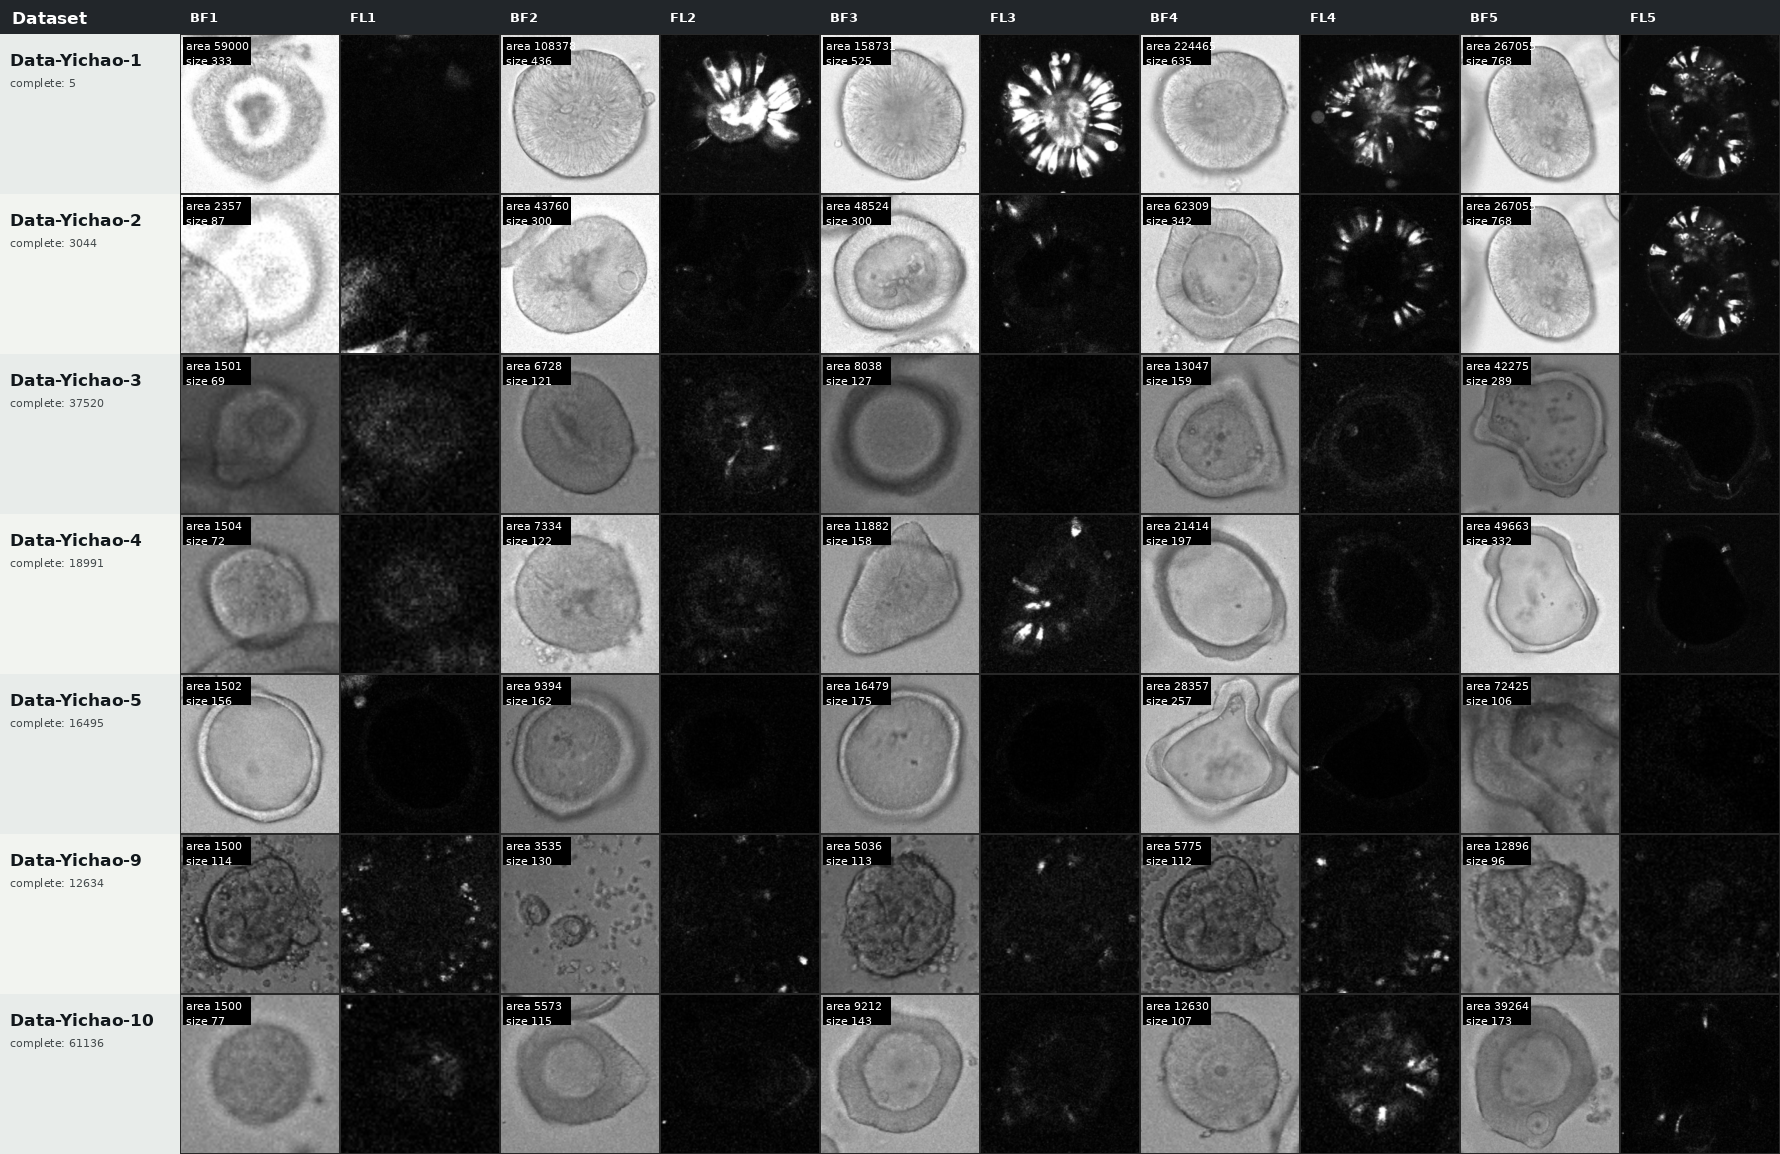
\includegraphics[width=\linewidth]{../../../visualizations/yichao_complete_instance_pair_grid_5_per_dataset.png}
}{
  \fbox{\parbox{0.85\linewidth}{Pair-grid image not found. Generate it from the resized-pair database before building this PDF.}}
}
\caption{Existing complete-organoid instance-pair visualization. Each dataset row shows paired brightfield/fluorescence crops for complete non-edge-padded organoids. This is a QC visualization, not yet a temporal forecast visualization.}
\label{fig:pair-grid}
\end{figure}

\subsection{Forecasting curve}
For each tracked organoid, plot:
\begin{equation}
\left\{(t,S_{j,t}), (t,\hat{y}_{j,t}^{\mathrm{pos}})\right\}_{t=1}^{T_j}.
\end{equation}
Overlay:
\begin{itemize}[leftmargin=1.5em]
  \item fluorescence threshold \(\theta_j\),
  \item detected onset \(\tau_j\),
  \item prefix endpoint \(k\),
  \item future target window.
\end{itemize}

This plot is the most important debugging visualization because it reveals whether the model is predicting before expression or merely reacting after expression has already begun.

\section{Concrete Demo Pipeline}
\subsection{Step 1: select time-aware data}
Use only folders where \(T>1\). In the current repository, the relevant grouped roots include:
\begin{verbatim}
Data-Yichao-v1/Data-Yichao-3/N39_TriRep_DF_jpeg_all_by_position
Data-Yichao-v1/Data-Yichao-4/N39_TriRep_DF_2_jpeg_all_by_position
Data-Yichao-v1/Data-Yichao-5/N39_TriRep_DF_3_jpeg_all_by_position
Data-Yichao-v1/Data-Yichao-6/N39_TriRep_4_jpeg_all_by_position
Data-Yichao-v1/Data-Yichao-7/N39_TriRep_5_jpeg_all_by_position
Data-Yichao-v1/Data-Yichao-8/N39_TriRep_DF_6_jpeg_all_by_position
Data-Yichao-v1/Data-Yichao-10/N39_TriRep_DF_7_jpeg_all_by_position
\end{verbatim}

\subsection{Step 2: build instance database}
The current segmentation pipeline writes:
\begin{verbatim}
analysis-outputs/yichao_instance_pairs/images/
analysis-outputs/yichao_instance_pairs/instances/
analysis-outputs/yichao_instance_pairs/database/instance_pairs.sqlite
\end{verbatim}

Use the database to filter complete organoids:
\begin{verbatim}
SELECT *
FROM instances
WHERE CAST(is_edge_padded AS INTEGER) = 0;
\end{verbatim}

\subsection{Step 3: create tracks}
Create a new track table:
\begin{verbatim}
tracks(track_id, dataset, object_name, time_index, z_index,
       instance_id, centroid_x, centroid_y, area_px,
       is_edge_padded, fluorescence_score, track_quality)
\end{verbatim}

For the first implementation, build one 2D representation per timepoint using a best-focus or projection rule.

\subsection{Step 4: create future labels}
Create a track-label table:
\begin{verbatim}
track_labels(track_id, future_positive, onset_time_index,
             future_peak, future_auc, censor_flag)
\end{verbatim}

\subsection{Step 5: train and visualize}
Train the variable-prefix model and produce:
\begin{itemize}[leftmargin=1.5em]
  \item prefix-length performance plot;
  \item prediction examples for high-confidence positive and negative tracks;
  \item onset curves with predicted risk;
  \item morphology feature importance.
\end{itemize}

\section{Future Image Prediction}
After scalar forecasting works, add an image decoder:
\begin{equation}
\hat{F}_{j,t+h}^{\mathrm{crop}}
=
D_\omega(h_{j,k}, h),
\end{equation}
where \(h\) is the forecast horizon. Train with mask-restricted image losses:
\begin{equation}
\mathcal{L}_{\mathrm{image}}
=
\left\|M_{j,t+h}\odot
\left(\hat{F}_{j,t+h}^{\mathrm{crop}}-F_{j,t+h}^{\mathrm{crop}}\right)
\right\|_1
\;+\;
\eta\,\mathcal{L}_{\mathrm{SSIM}}
\;+\;
\rho\,\mathcal{L}_{\mathrm{Dice}}.
\end{equation}

Do not start with this image task. It is harder because future organoid geometry is not fixed. The scalar future-expression model should be the first scientifically interpretable result.

\section{Main Risks and Controls}
\begin{itemize}[leftmargin=1.5em]
  \item \textbf{Tracking risk:} if same-organoid tracking is unreliable, switch to position-level forecasting.
  \item \textbf{Leakage risk:} do not allow weak fluorescence in the input prefix; use an onset guard.
  \item \textbf{Split risk:} split by position or LIF file, not by individual planes.
  \item \textbf{Artifact risk:} debris can have strong fluorescence; use morphology and complete-organoid masks to reject non-organoid objects.
  \item \textbf{Class imbalance:} if positive tracks are rare, report AUPRC and calibrate thresholds.
\end{itemize}

\section{Minimal First Experiment}
The first robust experiment should be:
\begin{itemize}[leftmargin=1.5em]
  \item data: complete tracked organoids from time-aware Yichao datasets;
  \item input: early brightfield crop sequence before onset;
  \item target: future positive, \(\log(1+\mathrm{peak})\), \(\log(1+\mathrm{AUC})\);
  \item model: CNN encoder plus morphology features plus GRU;
  \item split: held-out positions;
  \item decision: find the shortest prefix \(k^\star\) with near-best validation performance.
\end{itemize}

This directly answers whether early brightfield morphology can predict later differentiation-related fluorescence expression.

\end{document}
